\documentclass[12pt]{article}
\usepackage{amsmath, amssymb, amsfonts, bm, graphicx, geometry, tabularx, booktabs, float, enumitem, cancel}
\geometry{margin=1in}

\title{}
\date{}
\author{}

% Uppercase Volume with thicker, higher line
\newcommand{\vol}{\mathord{\text{\ooalign{\hidewidth $V$\hidewidth\cr\kern-0.5pt\raisebox{0.8ex}{\rule[0pt]{1em}{0.5pt}}}}}}

% Lowercase Volume with built-in shifts
\newcommand{\svol}{%
  \mathord{\text{\ooalign{%
    \hfil$v$\hfil\cr
    \hfil\rule[0.6ex]{0.8em}{0.5pt}\hfil
  }}}%
}

\begin{document}
\noindent
\section*{Notes}
\textbf{Ideal Gas Carnot Cycle}\\
Consider the following piston-cylinder system containing an ideal gas, which undergoes a Carnot cycle.
\begin{center}
    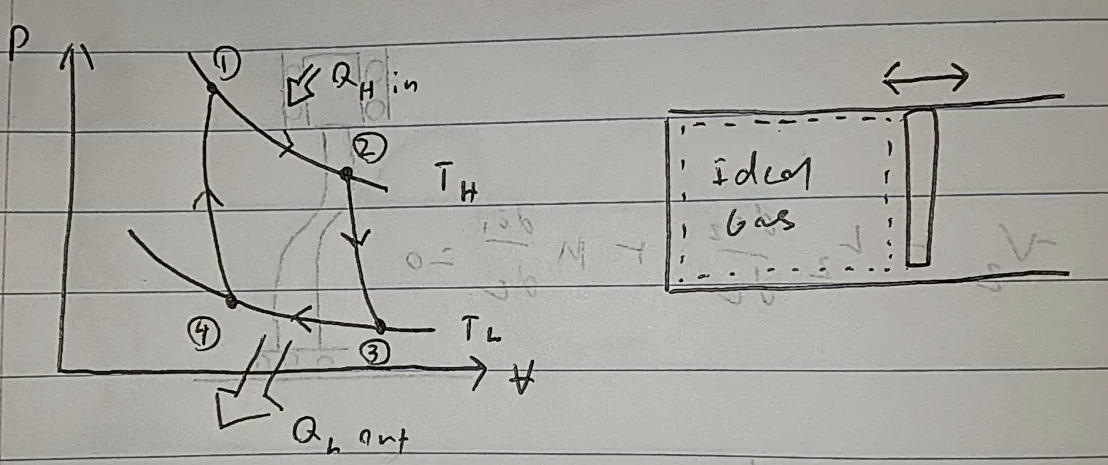
\includegraphics[width=0.7\textwidth]{ideal gas carnot.png}
\end{center}
Since it is a Carnot cycle, it consists of two isothermal ($dT=0$) processes and two adiabatic ($\delta Q = 0$) processes:
\begin{itemize}
    \item $1 \to 2$: Isothermal expansion at $T_H$ (Heat addition: $Q_H$)
    \item $2 \to 3$: Adiabatic expansion
    \item $3 \to 4$: Isothermal compression at $T_L$ (Heat rejection: $Q_L$)
    \item $4 \to 1$: Adiabatic compression
\end{itemize}
Applying the first law of thermodynamics to the ideal gas (a closed system):
\[du = \delta q - \delta w\]
We can use the following relations to rewrite the first law:
\[P\svol = RT\quad\text{(Ideal Gas Eqn of State)}\]
\[\delta w = Pd\svol\quad\text{(Work for Closed System)}\]
\[du=c_{\svol} dT \quad \text{(Constant Specific Heat)}\]
\[\implies \quad \boxed{\delta q = c_{\svol} dT+\frac{RT}{\svol}d\svol}\]
Applying this ODE to each process and integrating, we have useful relations for the adiabatic and isothermal processes:
\begin{itemize}
    \item Isothermal ($dT=0$): Processes $1 \to 2$ and $3 \to 4$
    \[\delta q = \frac{RT}{\svol} d\svol \implies \int_{1}^{2} \delta q = RT\int_{1}^{2} \frac{1}{\svol} d\svol\]
    \[\boxed{{}_1q_2 = RT\ln\left(\frac{\svol_2}{\svol_1}\right)}\]
    \underline{Note:} The temperature $T$ for this isothermal equation correlates to either $T_H$ or $T_C$ depending on the process.
    \newpage
    \item Adiabatic ($\delta q=0$): Processes $2 \to 3$ and $4 \to 1$
    \[0 = c_{\svol} dT+\frac{RT}{\svol}d\svol \implies \int_{1}^{2}\frac{1}{T}dT = \int_{1}^{2} -\frac{R}{c_{\svol}}\frac{d\svol}{\svol}\]
    \[\boxed{\ln\left(\frac{T_2}{T_1}\right) = -\frac{R}{c_{\svol}}\ln\left(\frac{\svol_2}{\svol_1}\right)}\]
    \underline{Note:} We assume that the specific heat $c_{\svol}$ is constant for this process, so we can choose $c_{\svol}$ at either $T_1$ or $T_2$ ($T_H$ or $T_C$) for this equation. However, if the temperature difference is LARGE, then \underline{use the average specific heat} ${c}_{\svol,\text{avg}} = \frac{c_{\svol}(T_1)+c_{\svol}(T_2)}{2}$ for better accuracy.
\end{itemize}
\textbf{Clausius Inequality}\\
Consider the following reversible Carnot cycle:
\begin{center}
    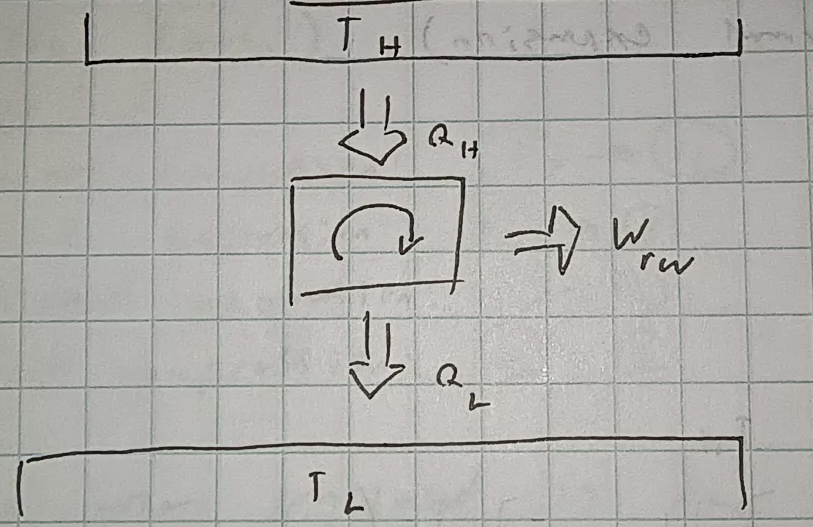
\includegraphics[width=0.5\textwidth]{rev carnot.png}
\end{center}
We can express the \textit{net} heat transfer for this cycle as:
\[\sum Q = Q_H - Q_L\quad \implies \oint \delta Q = Q_H - Q_L\]
Now consider the following modification: since the heat transfer only happens during \textit{isothermal} processes, we can write the following sum:
\[\sum \frac{Q}{T} = \frac{Q_H}{T_H} - \frac{Q_L}{T_L} \implies \oint \frac{\delta Q}{T} = \frac{Q_H}{T_H} - \frac{Q_L}{T_L}\]
Recall that for a reversible Carnot cycle:
\[\eta = \underbrace{1-\frac{Q_L}{Q_H}}_{\eta_{\text{HE}}} = \underbrace{1-\frac{T_L}{T_H}}_{\eta_{\text{Carnot,HE}}}\implies \frac{Q_H}{T_H} = \frac{Q_L}{T_L}\]
Thus, for a \underline{reversible process}:
\[\oint \frac{\delta Q}{T} = 0\]
Now compare to an \underline{irreversible} cycle:\\
By relating the actual efficiency of an irreversible cycle to the Carnot efficiency, we see that:
\[\eta_\text{HE} = \frac{W_\text{HE,actual}}{Q_H}=1 - \frac{Q_\text{}{L,actual}}{Q_H}< \eta_{\text{Carnot,HE}} = 1 - \frac{Q_L}{Q_H}\]
From the inequality, we can see that: $Q_\text{L,actual}< Q_L$. This makes sense because the irreversible cycle has more losses through $Q_{L,actual}$ such that the $W_\text{HE,actual}$ is smaller than the reversible case. \\\\
Writing the same sum for an irreversible cycle, we have:
\[\oint \frac{Q}{T} = \frac{Q_H}{T_H} - \frac{Q_{L,actual}}{T_L} < 0\]
Thus, for ALL \underline{irreversible processes}:
\[\oint \frac{\delta Q}{T} < 0\]
While this inequality was derived using the heat engine cycle, this applies to all cycles (including refrigerators and heat pumps) since they are just the same cycle in reverse. Clausius generalizes this as the following inequality for ALL cycles:
\[\boxed{\oint \frac{\delta Q}{T} \leq 0}\]
Where:
\begin{itemize}
    \item $\oint \frac{\delta Q}{T} = 0$ for reversible processes
    \item $\oint \frac{\delta Q}{T} < 0$ for irreversible processes
    \item $\oint \frac{\delta Q}{T} > 0$ is \textbf{impossible} since it violates the second law of thermodynamics
\end{itemize}
\textbf{Entropy as a State Property}\\
Previously we saw that:
\[\oint \left(\frac{\delta Q}{T}\right)_\text{rev} = 0\]
Mathematically, if the integral of a quantity is zero for all closed paths, then it is path independent and thus a state property (it only depends on the state/end points). Thus, we can define a new state property called \textbf{entropy} $S$ such that:
\[\Delta S = S_2-S_1 = \int_1^2 \left(\frac{\delta Q}{T}\right)_\text{rev}\]
\[\implies \quad \boxed{dS \equiv \left(\frac{\delta Q}{T}\right)_\text{rev}}\]
It has units of [kJ/K] or for specific entropy $s$ [kJ/kg$\cdot$K].\\\\
However, this is only defined for a reversible process, so to generalize this to an irreversible process, we can use the Clausius inequality:
\[\oint \frac{\delta Q}{T} < 0 \]
To account for the irreversibility, we add an extra term $S_\text{gen}$ for the entropy \textit{generated}. Thus, generally for any process (reversible or irreversible), \textbf{the entropy statement of the second law of thermodynamics} is:
\[S_2 - S_1 = \int_{1}^{2} \frac{\delta Q}{T} + {}_1S_{2\text{ gen}}\]
Where:
\begin{itemize}
    \item ${}_1S_{2\text{ gen}}=0$ for reversible processes
    \item ${}_1S_{2\text{ gen}}>0$ for irreversible processes
    \item ${}_1S_{2\text{ gen}}<0$ is \textbf{impossible} since it violates the second law of thermodynamics (entropy cannot be destroyed)
\end{itemize}
When applied to an actual system, we note where these variables correspond to:
\[\boxed{S_2 - S_1 = \int_{1}^{2} \left(\frac{\delta Q}{T}\right)_\text{CS} + {}_1S_{2\text{ gen}},\quad {}_1S_{2\text{ gen}}\geq 0 }\]
In rate form, this is:
\[\boxed{\frac{dS_\text{CM}}{dt} = \frac{\dot{Q}}{T_\text{CS}}+\dot{S}_\text{gen},\quad \dot{S}_\text{gen}\geq 0}\]
Where:
\begin{itemize}
    \item $\int_{1}^{2} \left(\frac{\delta Q}{T}\right)_\text{CS}$ is the entropy transfer across the \textit{control surface} boundary via heat transfer. The temperature used here is the temperature at the control surface, which is the temperature of the system at the boundary where heat transfer occurs.
    \item $\frac{dS_\text{CM}}{dt}$ is the rate at which entropy changes within the \textit{control mass} (closed system).
    \item $\frac{\dot{Q}}{T_\text{CS}}$ is the rate of entropy transfer across the control surface boundary via heat transfer.
\end{itemize}
\textbf{Temperature-Entropy (T-S) Plots}\\
Note that like any other property, we can obtain the value of entropy for a given state as long as we know two other properties:
\begin{center}
    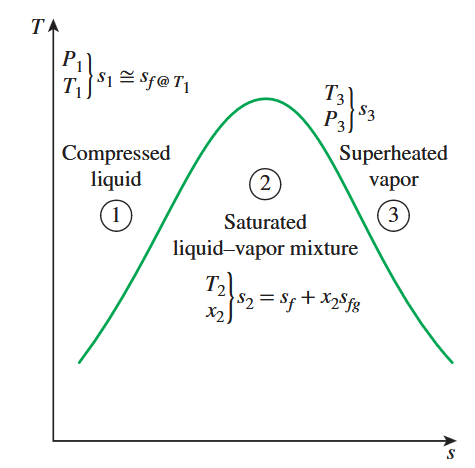
\includegraphics[width=0.5\textwidth]{entropy property.png}
\end{center}
Note that the \textit{condensed liquid approximation} and quality of a saturated mixture is used the same way for entropy as it is for other properties.\\\\
The T-S plot for water is shown below:
\begin{center}
    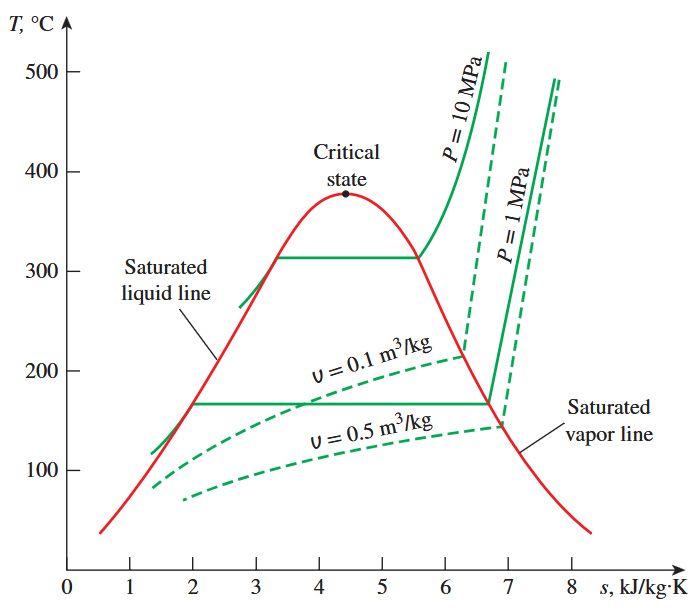
\includegraphics[width=0.7\textwidth]{TS more like tspmo.png}
\end{center}
We can ignore the constant volume lines. Note that for superheated substances, like the $P-\vol$ plot, we only show the right region of the T-S plot.\\\\
We have to be careful when plotting states on a T-S plot since a single isotherm intersects multiple isobars, thus we need to either specify the pressure or phase of the substance to plot the correct point.\\\\
\textbf{Heat Transfer from T-S Plot}\\
Recall that for a \underline{reversible} process, entropy is defined as:
\[dS = \left(\frac{\delta Q}{T}\right)_\text{rev}\]
\[\implies \boxed{Q = \int TdS\quad \text{(area under the T-S plot)}}\]
\textbf{Reversible Carnot Cycle on T-S Plot}\\
On a T-S plot, an isothermal process is a horizontal line (since $T$ is constant), while an adiabatic process is a vertical line (since $Q=\int TdS = 0$). Thus, the reversible Carnot cycle on a T-S plot looks like the following:
\begin{center}
    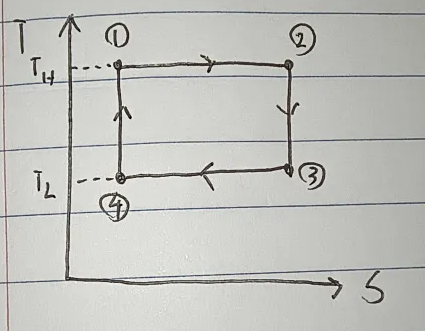
\includegraphics[width=0.5\textwidth]{carnot TS.png}
\end{center}
The area enclosed by the cycle is \textit{equal} to the net work done by the cycle (shown by the area enclosed by the P-$\vol$ plot) for a \textit{reversible process}. This is because:
\begin{center}
    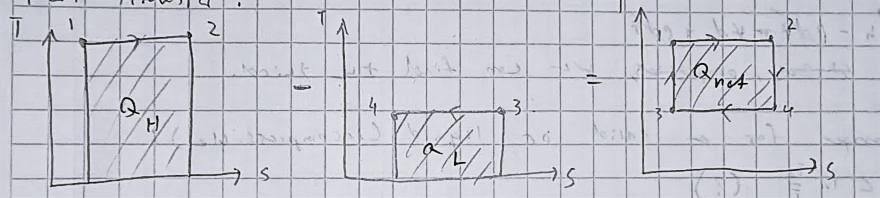
\includegraphics[width=0.7\textwidth]{net heat transfer carnot.png}
\end{center}
and by energy conservation, $W_\text{net} = Q_\text{net}$ for a cycle.\\\\
\newpage\noindent
\textbf{Entropy Change for a Phase Change}\\
Consider the following phase change process from a saturated liquid to a saturated vapor:
\begin{center}
    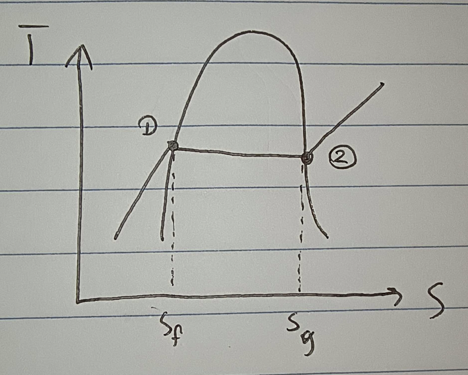
\includegraphics[width=0.4\textwidth]{phase.png}
\end{center}
Since this is a phase change, the temperature stays at the constant saturation temperature $T_\text{sat}$. From the first law for a closed system, we have:
\[du = \delta q - dw \implies {}_1q_2 = u_2-u_1 +P(\svol_2-\svol_1)\]
Since enthalpy is defined as $h = u + P\svol$, we can rewrite the above equation as:
\[\implies {}_1q_2 = h_2 - h_1 = h_\text{fg}\]
Now we can relate heat transfer to entropy change for reversible processes:
\[s_2 - s_1 =\int_{1}^{2} \left(\frac{\delta Q}{T}\right)_\text{rev}=\frac{{}_1q_2}{T_\text{sat}}\]
\[\implies \boxed{s_\text{fg} = \frac{h_\text{fg}}{T_\text{sat}}}\]
\section*{Gibbs Relations}
These relationships are especially powerful because it allows us to relate entropy to other state properties, and it applies to ALL processes, not limited to cycles or reversible processes!\\\\
Begin with the first law of thermodynamics:
\[du = \delta q - dw\]
We can rewrite the first law using the following relations:
\[\delta q = Tds\quad \text{(definition of entropy)}\]
\[\delta w = Pd\svol\quad \text{(work for closed system)}\]
\[\implies du = Tds - Pd\svol\]
The first Gibbs relation is then:
\[\boxed{Tds = du + Pd\svol\quad \text{(First Gibbs Relation)}}\]
For open systems or constant pressure processes, we can rewrite the first Gibbs relation using the definition of enthalpy $h = u + P\svol$ to get the second Gibbs relation:
\[dh = du+Pd\svol+\svol dP \implies du= dh - Pd\svol-\svol dP\]
\[\boxed{Tds = dh - \svol dP\quad \text{(Second Gibbs Relation)}}\]
\textbf{Applying Gibbs Relations to Ideal Gas}\\
For an ideal gas, we have the following relations:
\[P\svol = RT\]
\[du = C_{\svol0}dT\]
\[dh = C_{P0}dT\]
Where $C_{\svol0}$ and $C_{P0}$ are the constant specific heats.\\\\
Applying the first Gibbs relation to an ideal gas, we have:
\[\boxed{ds =\frac{C_{\svol0}}{T}dT+\frac{R}{\svol}d\svol \implies s_2-s_1 = C_{\svol0}\ln\left(\frac{T_2}{T_1}\right)+R \ln\left(\frac{\svol_2}{\svol_1}\right) \quad \text{(From First Gibbs Relation)}}\]
Applying the second Gibbs relation to an ideal gas, we have:
\[\boxed{ds = \frac{C_{P0}}{T}dT-\frac{R}{P}dP \implies s_2-s_1 = C_{P0}\ln\left(\frac{T_2}{T_1}\right)-R \ln\left(\frac{P_2}{P_1}\right) \quad \text{(From Second Gibbs Relation)}}\]
Note that these two equations are equivalent since $C_{P0} = C_{\svol0} + R$ for an ideal gas.\\\\
\textbf{Variable Specific Heat}\\
Before we assumed that the specific heat is constant, but a more accurate model is to assume that the specific heat is a function of temperature. Using the \textbf{standard entropy} $s_T^0$ at a temperature $T$, we can rewrite the Gibbs relations for an ideal gas with variable specific heat as:
\[\boxed{s_2-s_1 = s_{T_2}^0 - s_{T_1}^0 - R \ln\left(\frac{P_2}{P_1}\right) \quad \text{(From Second Gibbs Relation)}}\]
\textbf{Absolute Entropy}\\
Using a reference state at $T=0$ K and $P_0 = 1$ atm, we can define the \textbf{absolute entropy} as:
\[\boxed{s(T,P) = s_T^0-R\ln\left(\frac{P}{P_0}\right)}\]
\section*{Entropy Balance}
For a closed system, we can write the entropy balance as:
\[\boxed{\sum \frac{Q_k}{T_k}+S_{\text{gen}}=\Delta S_{\text{sys}} \quad [\text{kJ/K}]}\]
Where $Q_k$ is the heat transfer across the system boundary at temperature $T_k$, and $S_\text{gen}$ is the entropy generated within the system.\\\\
For an open system, we can write the entropy balance as:
\[\boxed{\sum \frac{\dot{Q}_k}{T_k} +\sum \dot{m}_i s_i - \sum \dot{m}_e s_e + \dot{S}_\text{gen} = \frac{dS_\text{CV}}{dt} \quad [\text{kW/K}]}\]
\section*{7-24}
\vspace{-2em}
\begin{center}
    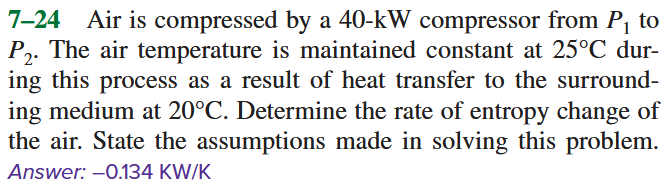
\includegraphics[width=0.7\textwidth]{7-24.png}
\end{center}
Given:
\begin{itemize}
    \item $\dot{W} = -40$ kW (power input to the compressor)
    \item $T = 25^\circ$C (Constant temperature: isothermal process)
    \item Surroundings at $T_\text{sur} = 20^\circ$C 
    \item Change in pressure: $P_2-P_1$
    \item Air
\end{itemize}
Starting from the entropy balance for an open system (CV: air in the compressor):
\[\sum \frac{\dot{Q}_k}{T_k} +\sum \dot{m}_i s_i - \sum \dot{m}_e s_e + \dot{S}_\text{gen} = \frac{dS_\text{CV}}{dt}\]
Simplifying the entropy balance using the following assumptions:
\begin{itemize}
    \item Steady state: $\frac{dS_\text{CV}}{dt} = 0$. Similar to the intuition for steady state in the first law, there is no accumulation of mass, thus there is no accumulation of entropy in the system.
    \item Single inlet and single outlet: by the conservation of mass, $\dot{m}_i = \dot{m}_e$, so we can write the mass flow rate as $\dot{m}$.
    \item Assuming that the process is reversible, we have $\dot{S}_\text{gen} = 0$. This is because the problem states that the process is an isothermal compression and it doesn't specify any irreversibilities.    
    \item $\sum \frac{\dot{Q}_k}{T_k} = \frac{\dot{Q}}{T_\text{air}}$ because there is only one heat transfer across the air boundary.
\end{itemize}
Thus, the entropy balance simplifies to:
\[\frac{\dot{Q}}{T_\text{air}} - \underbrace{\dot{m}(s_e - s_i)}_{\Delta \dot{S}_\text{air}} = 0\]
\[\implies \Delta \dot{S}_\text{air} = \frac{\dot{Q}}{T_\text{air}}
\]
Applying the first law of thermodynamics to the air in the compressor:
\[\frac{dE}{dt} = \dot{Q} - \dot{W} +\sum \dot{m}_i \left[h_i +\frac{1}{2}V_i^2 + gz_i\right] - \sum \dot{m}_e \left[h_e +\frac{1}{2}V_e^2 + gz_e\right]\]
We can simplify the first law using the following assumptions:
\begin{itemize}
    \item Steady state: $\frac{dE}{dt} = 0$. 
    \item Single inlet and single outlet: by the conservation of mass, $\dot{m}_i = \dot{m}_e$, so we can write the mass flow rate as $\dot{m}$.
    \item Negligible kinetic and potential energy changes: $\frac{1}{2}V_i^2 \approx \frac{1}{2}V_e^2 \approx 0$ and $gz_i \approx gz_e \approx 0$.
\end{itemize}
Thus, the first law simplifies to:
\[0 = \dot{Q} - \dot{W} + \dot{m}(h_1 - h_2)\]
Assuming a constant specific heat capacity for air:
\[h_2 - h_1 = c_p (T_2 - T_1)\]
Since the process is isothermal, $T_2 = T_1$, thus $h_2 - h_1 = 0$. Therefore, the first law simplifies to:
\[\dot{Q} = \dot{W} = [-40 \text{ kW}]\]
Finally, plugging this into the entropy balance, we have:
\[T_\text{sur} = 25^\circ\text{C} + 273.15 = 298.15 \text{ K}\]
\[\Delta \dot{S}_\text{air} = \frac{\dot{Q}}{T_\text{sur}} = \frac{[-40 \text{ kW}]}{[298.15 \text{ K}]} = \boxed{-0.134 \text{ kW/K}}\]


\newpage
\section*{7-93}
\vspace{-2em}
\begin{center}
    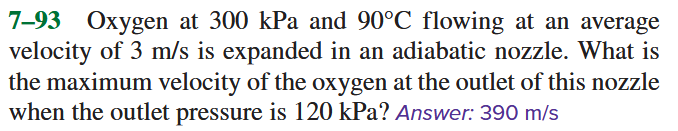
\includegraphics[width=0.7\textwidth]{7-93.png}
\end{center}
Given:
\begin{itemize}
    \item Oxygen gas
    \item State 1:
    \begin{itemize}
        \item $P_1 = 300$ kPa
        \item $T_1 = 90^\circ$C
        \item $v_1 = 3$ m/s
    \end{itemize} 
    \item State 2:
    \begin{itemize}
        \item $P_2 = 120$ kPa
    \end{itemize}
    \item Adiabatic expansion ($\delta q = 0$)
\end{itemize}
Find: 
\begin{itemize}
    \item Maximum velocity of oxygen at the outlet of the nozzle ($v_2$)
\end{itemize}
First, from the entropy balance for the nozzle, we have:
\[\sum \frac{\dot{Q}_k}{T_k} +\sum \dot{m}_i s_i - \sum \dot{m}_e s_e + \dot{S}_\text{gen} = \frac{dS_\text{CV}}{dt}\]
However, because:
\begin{itemize}
    \item The process is adiabatic, so $\sum \frac{\dot{Q}_k}{T_k} = 0$.
    \item The process is steady state, so $\frac{dS_\text{CV}}{dt} = 0$.
    \item There is only one inlet and one outlet, so we can write the mass flow rate as $\dot{m}$.
    \item Assuming that there are no irreversibilities to calculate the ideal maximum velocity, we have $\dot{S}_\text{gen} = 0$.
\end{itemize}
Thus, the entropy balance shows that the process is \textit{isentropic}:
\[s_i = s_e\]
Assuming that the oxygen behaves like an ideal gas, we can apply the second Gibbs relation to find the temperature at state 2:
\[s_2 - s_1 = 0 = C_{p0}\ln\left(\frac{T_2}{T_1}\right) - R\ln\left(\frac{P_2}{P_1}\right)\]
\[\implies \frac{T_2}{T_1} = \exp\left(\frac{R}{C_{p0}}\ln\left(\frac{P_2}{P_1}\right)\right) = \left(\frac{P_2}{P_1}\right)^{\frac{R}{C_{p0}}}\]
Where at 300 K, $C_{p0} = 0.918$ kJ/kg$\cdot$K and $R = 0.2598$ kJ/kg$\cdot$K for oxygen and $T_1 = 90^\circ$C = 363.15 K. Thus, we have:
\[T_2 = [363.15\text{ K}]\left(\frac{[120\,\text{kPa}]}{[300\,\text{kPa}]}\right)^{\frac{0.2598}{0.918}}=[280.19\text{ K}]\]
Now we can apply the first law of thermodynamics to the nozzle:
\[\frac{dE}{dt} = \dot{Q} - \dot{W} +\sum \dot{m}_i \left[h_i +\frac{1}{2}V_i^2 + gz_i\right] - \sum \dot{m}_e \left[h_e +\frac{1}{2}V_e^2 + gz_e\right]\]
We can simplify the first law using the following assumptions:
\begin{itemize}
    \item Steady state: $\frac{dE}{dt} = 0$. 
    \item Single inlet and single outlet: by the conservation of mass, $\dot{m}_i = \dot{m}_e$, so we can write the mass flow rate as $\dot{m}$.
    \item Negligible potential energy changes: $gz_i \approx gz_e \approx 0$.
    \item No work done by the nozzle: $\dot{W} = 0$
    \item Adiabatic process: $\dot{Q} = 0$
\end{itemize}
Thus, the first law simplifies to:
\[0 =\dot{m}(h_1 - h_2) + \frac{1}{2}\dot{m}(V_1^2 - V_2^2)\]
\[V_2^2  = -2(h_1 - h_2) + V_1^2\]
Assuming a constant specific heat capacity for oxygen, we have:
\[h_2 - h_1 = C_p (T_2 - T_1)\]
Where $T_1 = 90^\circ$C = 363.15 K and $280.19\text{ K}$. Thus,
\[h_2 - h_1 = [0.918 \text{ kJ/kg$\cdot$K}] \cdot [(363.15 - 280.19) \text{ K}] = 76.157 \text{ kJ/kg}\]
Plugging this into the equation for $V_2^2$, we have:
\[V_2^2 = -2\left[-(76.157)\,\frac{\text{kJ}}{\text{kg}}\cdot\frac{10^3\,\text{kg}\cdot\text{m}^2/\text{s}^2}{\text{kJ}}\right] + [3 \text{ m/s}]^2 =152323.5 \text{ m}^2/\text{s}^2\]
\[\implies \boxed{V_2 = 390.2 \text{ m/s}}\]

\section*{7-107}
\vspace{-2em}
\begin{center}
    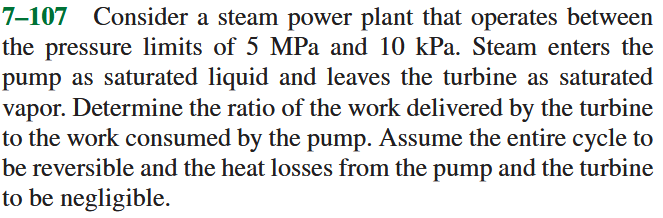
\includegraphics[width=0.7\textwidth]{7-107.png}
\end{center}
Given:
\begin{itemize}
    \item Steam power plane: Heat engine cycle with steam
    \item Pressure limits: 5 MPa, 10 kPa
    \item Steam enters the pump as a saturated liquid and leaves the turbine as a saturated vapor
    \item Reversible processes
    \item Negligible heat loss from pump and turbine: Adiabatic processes
\end{itemize}
Find:
\begin{itemize}
    \item Ratio of work out from turbine to work input to pump ($\frac{W_\text{turbine}}{W_\text{pump}}$)
\end{itemize}
\begin{center}
    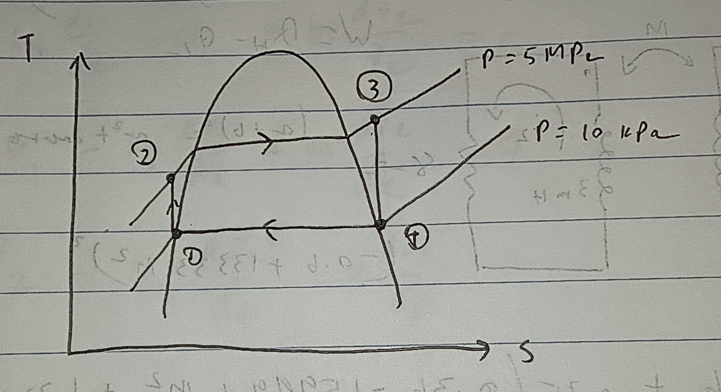
\includegraphics[width=0.6\textwidth]{7-107-1.png}
\end{center}
For the work input to the pump, we can apply the first law of thermodynamics to the pump:
\[\frac{dE}{dt} = \dot{Q} - \dot{W} +\sum \dot{m}_i \left[h_i +\frac{1}{2}V_i^2 + gz_i\right] - \sum \dot{m}_e \left[h_e +\frac{1}{2}V_e^2 + gz_e\right]\]
Simplify the first law by: steady state ($\frac{dE}{dt} = 0$), single inlet and outlet ($\dot{m}_i = \dot{m}_e = \dot{m}$), negligible kinetic and potential energy changes ($\frac{1}{2}V_i^2 \approx \frac{1}{2}V_e^2 \approx 0$ and $gz_i \approx gz_e \approx 0$), and adiabatic process ($\dot{Q} = 0$):
\[0 = -\dot{W} + \dot{m}(h_1 - h_2)\]
\[\implies \dot{W}_\text{pump} = \dot{m}(h_1 - h_2)\]
To find the change in enthalpy, we can use the Gibbs relations since this is a reversible adiabatic process, it is also isentropic.
\[Tds = dh - \svol dP \implies dh = \svol dP\]
\[h_2 - h_1 = \svol_1 (P_2 - P_1)\]
\textbf{State 1:} Pump inlet (saturated liquid at 10 kPa)
\[\svol_1 = \svol_f = 0.001010 \text{ m$^3$/kg}\]
\[h_1 = h_f = 191.81 \text{ kJ/kg}\]
\textbf{State 2:} Pump outlet (compressed liquid at 5 MPa)
\[\svol_2 \approx \svol_1 = 0.001010 \text{ m$^3$/kg}\quad\text{(water is incompressible)}\]
Thus, the pump work is:
\[\dot{W}_\text{pump} = \dot{m}(h_1 - h_2) = \dot{m}\svol_1 (P_1 - P_2) = \dot{m} [0.001010 \text{ m$^3$/kg}] \cdot [(10\times10^3 - 5\times10^6) \text{ Pa}] = \dot{m} [-5.03 \text{ kJ/kg}]\]
\[\implies W_\text{pump} = m[-5.03 \text{ kJ/kg}]\]
For the work output from the turbine, we can apply the first law of thermodynamics to the turbine with the same assumptions as the pump, getting:
\[\dot{W}_\text{turbine} = \dot{m}(h_3 - h_4)\]
\textbf{State 4:} Turbine exit (saturated vapor at 10 kPa)
\[h_4 = h_g = 2583.9 \text{ kJ/kg}\]
\[s_4 = s_g = 8.1488 \text{ kJ/kg$\cdot$K}\]
\textbf{State 3:} Turbine inlet (superheated vapor at 5 MPa)\\
To find $h_3$, we can use the superheated water tables with the following inputs: $P_3 = 5$ MPa and $s_3 = s_4 = 8.1488$ kJ/kg$\cdot$K (isentropic process). 
\[h_3 \approx h_{s=8.16}=4628.3 \text{ kJ/kg}\]
Thus, the turbine work is:
\[\dot{W}_\text{turbine} = \dot{m}(h_3 - h_4) = \dot{m} [4628.3 - 2583.9 \text{ kJ/kg}] = \dot{m} [2044.4 \text{ kJ/kg}]\]
\[\implies W_\text{turbine} = m[2044.4 \text{ kJ/kg}]\]
Finally, we can find the ratio of work output from the turbine to work input to the pump:
\[\left|\frac{W_\text{turbine}}{W_\text{pump}}\right| = \left|\frac{m[2044.4 \text{ kJ/kg}]}{m[-5.03 \text{ kJ/kg}]}\right| = \boxed{406.4}\]

\section*{7-117E}
\vspace{-2em}
\begin{center}
    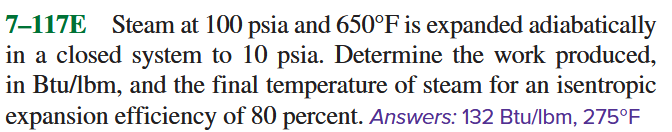
\includegraphics[width=0.7\textwidth]{7-117E.png}
\end{center}
Given:
\begin{itemize}
    \item Steam under an adiabatic expansion process (closed system)
    \item State 1: $P_1 = 100$ psia, $T_1 = 650^\circ$F
    \item State 2: $P_2 = 10$ psia
    \item Isentropic expansion efficiency $\eta = 0.8$
\end{itemize}
Find:
\begin{itemize}
    \item Work produced [Btu/lbm]
    \item Final temperature $T_2$ [F]
\end{itemize}
For a closed system, we can apply the first law of thermodynamics:
\[\Delta U = Q - W\]
Since the process is adiabatic, $Q=0$, thus:
\[\Delta U = -W\]
\[\implies W = -m(u_2 - u_1)\]
\textbf{State 1:} $P_1 = 100$ psia, $T_1 = 650^\circ$F\\
From the superheated steam tables, we can find the specific internal energy at state 1 through linear interpolation. Using the following values:
\begin{itemize}
    \item $T=600^\circ$F: $u_{600} = 1214.4$ Btu/lbm
    \item $T=700^\circ$F: $u_{700} = 1253.0$ Btu/lbm
\end{itemize}
\[u-u_{600} = \frac{u_{700}-u_{600}}{T_{700}-T_{600}}(T-T_{600})\]
\[u = 1214.4 +0.386(T-600)\quad \implies u_1 = 1233.7 \text{ Btu/lbm}\]
We can also find the specific entropy at state 1 through linear interpolation. Using the following values:
\begin{itemize}
    \item $T=600^\circ$F: $s_{600} = 1.7586$ Btu/lbm$\cdot$R
    \item $T=700^\circ$F: $s_{700} = 1.8037$ Btu/lbm$\cdot$R
\end{itemize}
\[s-s_{600} = \frac{s_{700}-s_{600}}{T_{700}-T_{600}}(T-T_{600})\]
\[s = 1.7586+0.000451(T-600)\quad \implies s_1 = 1.781 \text{ Btu/lbm$\cdot$R}\]
\textbf{State 2:} $P_2 = 10$ psia\\
Since the process is isentropic: $s_2 = s_1 = 1.781$ Btu/lbm$\cdot$R. From the saturated water tables at $P_2 = 10$ psia, we see that $s_f<s_2<s_g$, thus state 2 is a saturated mixture. We can find the quality of the saturated mixture at state 2:
\[x = \frac{s_2 - s_f}{s_{fg}} = \frac{[1.781-0.28362\text{ Btu/lbm$\cdot$R} ]}{[1.50391\text{ Btu/lbm$\cdot$R}]}=0.995\]
Now we can find the specific internal energy at state 2:
\[u_2 = u_f + x u_{fg} = [161.22\text{ Btu/lbm}] + 0.995 \cdot [910.75\text{ Btu/lbm}] = 1067.416 \text{ Btu/lbm}\]
Finally, we can find the work produced by the adiabatic expansion process:
\[W = -m(u_2 - u_1) = m[166.284 \text{ Btu/lbm}]\]
Applying the isentropic expansion efficiency, we have:
\[w_\text{actual} = \eta w_\text{isentropic} = 0.8 \cdot [166.284 \text{ Btu/lbm}] = \boxed{133.027 \text{ Btu/lbm}}\]
\textbf{Finding the temperature}\\
Since we find that the actual work done is slightly less, we can find the actual internal energy at state 2:
\[W_\text{actual} = m(u_1 - u_2) = m[133.027 \text{ Btu/lbm}]\]
\[\implies u_2 = [1233.7\, \text{Btu/lbm}] - [133.027\, \text{Btu/lbm}] = 1100.673\, \text{Btu/lbm}\]
Looking at the property tables at $P_2 = 10$ psia, we see that $u_g<u_2$, thus state 2 is a superheated vapor. From the superheated steam tables at $P_2 = 10$ psia, we can find the temperature at state 2 through linear interpolation. Using the following values:
\begin{itemize}
    \item $T=240^\circ$F: $u_{240} = 1089.1$ Btu/lbm
    \item $T=280^\circ$F: $u_{280} = 1103.4$ Btu/lbm
\end{itemize}
\[T-T_{240} = \frac{T_{280}-T_{240}}{u_{280}-u_{240}}(u-u_{240})\]
\[T= 240 + 2.797(u-1089.1)\quad\implies T_2 = \boxed{272.37^\circ\text{F}}\]
\newpage
\section*{7-136}
\vspace{-2em}
\begin{center}
    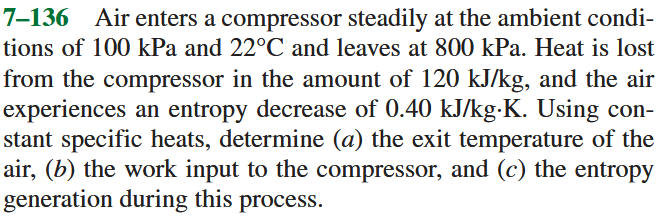
\includegraphics[width=0.7\textwidth]{7-136.png}
\end{center}
Given:
\begin{itemize}
    \item Air enters a compressor at steady state
    \item State 1: $P_1 = 100$ kPa, $T_1 = 22^\circ$C
    \item State 2: $P_2 = 800$ kPa
    \item $Q = -120$ kJ/kg
    \item $\Delta s = -0.4$ kJ/kg$\cdot$K
    \item Use constants specific heat capacities 
\end{itemize}
Find:
\begin{itemize}
    \item Exit temperature $T_2$ [K]
    \item Work input to the compressor $W$ [kJ/kg]
    \item Entropy generated $s_\text{gen}$ [kJ/kg$\cdot$K]
\end{itemize}
\textbf{Exit Temperature}\\
We can use the second Gibbs relation to find the exit temperature:
\[s_2-s_1 = [-0.4\text{ kJ/kg$\cdot$K}]= c_{p0}\ln\left(\frac{T_2}{T_1}\right) - R\ln\left(\frac{P_2}{P_1}\right)\]
Where at 300 K, $c_{p0} = 1.005$ kJ/kg$\cdot$K and $R = 0.2870$ kJ/kg$\cdot$K for air. Thus solving for $T_2$, we have:
\[\frac{T_2}{T_1} = \exp\left(\frac{R}{c_{p0}}\ln\left(\frac{P_2}{P_1}\right) + \frac{[-0.4\text{ kJ/kg$\cdot$K}]}{c_{p0}}\right)\]
\[\frac{T_2}{T_1} = \exp\left(\frac{[0.2870\text{ kJ/kg$\cdot$K}]}{[1.005\text{ kJ/kg$\cdot$K}]}\ln\left(\frac{[800\text{ kPa}]}{[100\text{ kPa}]}\right) + \frac{[-0.4\text{ kJ/kg$\cdot$K}]}{[1.005\text{ kJ/kg$\cdot$K}]}\right) = 1.216\]
For $T_1 = 22^\circ$C = 295.15 K, we have:
\[T_2 = [295.15\text{ K}] \cdot 1.216 = \boxed{358.8\text{ K}}\]
\textbf{Work Input}\\
We can apply the first law of thermodynamics to the compressor to find the work input:
\[\frac{dE}{dt} = \dot{Q} - \dot{W} +\sum \dot{m}_i \left[h_i +\frac{1}{2}V_i^2 + gz_i\right] - \sum \dot{m}_e \left[h_e +\frac{1}{2}V_e^2 + gz_e\right]\]
This simplifies: steady state ($\frac{dE}{dt} = 0$), single inlet and outlet ($\dot{m}_i = \dot{m}_e = \dot{m}$), negligible kinetic and potential energy changes ($\frac{1}{2}V_i^2 \approx \frac{1}{2}V_e^2 \approx 0$ and $gz_i \approx gz_e \approx 0$):
\[0 = \dot{Q} - \dot{W} + \dot{m}(h_1 - h_2)\]
Integrating over time and dividing by mass, we have:
\[w = q + (h_1 - h_2)\]
Assuming a constant specific heat capacity for air, we have:
\[h_2 - h_1 = c_p (T_2 - T_1)\]
Where $T_1 = 295.15$ K and $T_2 = 358.8$ K. Thus, we have:
\[w = q + c_p (T_1 - T_2) = [-120\text{ kJ/kg}]+[1.005\text{ kJ/kg$\cdot$K}][295.15 - 358.8\text{ K}] = \boxed{-183.96\text{ kJ/kg}}\]
\textbf{Entropy Generated}\\
Using the entropy balance for an open system, we have:
\[\sum \frac{\dot{Q}_k}{T_k} +\sum \dot{m}_i s_i - \sum \dot{m}_e s_e + \dot{S}_\text{gen} = \frac{dS_\text{CV}}{dt}\]
This simplifies: steady state ($\frac{dS_\text{CV}}{dt} = 0$), single inlet and outlet ($\dot{m}_i = \dot{m}_e = \dot{m}$):
\[\frac{\dot{Q}}{T_\text{ambient}} + \dot{m}(s_1 - s_2) + \dot{S}_\text{gen} = 0\]
Integrating over time and dividing by mass, we have:
\[s_\text{gen} = -\frac{q}{T_\text{ambient}} - (s_1 - s_2) = -\frac{[-120\text{ kJ/kg}]}{[295.15\text{ K}]} - [0.4\text{ kJ/kg$\cdot$K}] = \boxed{0.0065\text{ kJ/kg$\cdot$K}}\]
\newpage
\section*{7-175}
\vspace{-2em}
\begin{center}
    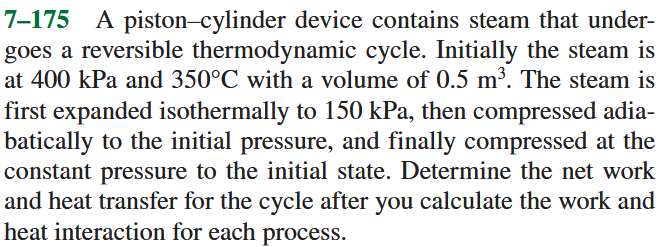
\includegraphics[width=0.7\textwidth]{7-175.png}
\end{center}
Given:
\begin{itemize}
    \item Piston-cylinder device with steam undergoing a reversible cycle
    \item State 1: $P_1 = 400$ kPa, $T_1 = 350^\circ$C, $\vol_1 = 0.5$ m$^3$
    \item Isothermal expansion from state 1 to state 2
    \item State 2: $P_2 = 150$ kPa
    \item Adiabatic compression from state 2 to state 3
    \item State 3: $P_3 = P_1 = 400$ kPa
    \item Isobaric compression from state 3 to state 1
\end{itemize}
Find:
\begin{itemize}
    \item Work and heat transfer for each process
    \item Net work and heat transfer for the cycle
\end{itemize}
\textbf{State 1:} $P_1 = 400$ kPa, $T_1 = 350^\circ$C, $\vol_1 = 0.5$ m$^3$\\
From the superheated steam tables, we can find the specific volume using linear interpolation with the following values:
\begin{itemize}
    \item $T=300^\circ$C: $\svol_{300} = 0.65489$ m$^3$/kg
    \item $T=400^\circ$C: $\svol_{400} = 0.77265 $ m$^3$/kg
\end{itemize}
\[\svol-\svol_{300} = \frac{\svol_{400}-\svol_{300}}{T_{400}-T_{300}}(T-T_{300})\]
\[\svol = 0.65489 + 0.001177(T-300)\quad \implies \underline{\svol_1 = 0.71377 \text{ m$^3$/kg}}\]
Now we can find the mass of the steam:
\[m = \frac{\vol_1}{\svol_1} = \frac{[0.5\text{ m$^3$}]}{[0.71377 \text{ m$^3$/kg}]} = \underline{0.7005 \text{ kg}}\]
Internal energy:
\begin{itemize}
    \item $T=300^\circ$C: $u_{300} = 2805.1$ kJ/kg
    \item $T=400^\circ$C: $u_{400} = 2964.9 $ kJ/kg
\end{itemize}
\[u-u_{300} = \frac{u_{400}-u_{300}}{T_{400}-T_{300}}(T-T_{300})\]
\[u = 2805.1 + 1.598(T-300)\quad \implies \underline{u_1 = 2885 \text{ kJ/kg}} \]
Entropy:
\begin{itemize}
    \item $T=300^\circ$C: $s_{300} = 7.5677$ kJ/kg$\cdot$K
    \item $T=400^\circ$C: $s_{400} = 7.9003 $ kJ/kg$\cdot$K
\end{itemize}
\[s-s_{300} = \frac{s_{400}-s_{300}}{T_{400}-T_{300}}(T-T_{300})\]
\[s = 7.5677 + 0.0033(T-300)\quad \implies \underline{s_1 = 7.734 \text{ kJ/kg$\cdot$K}}\]
\textbf{State 2:} $P_2 = 150$ kPa\\
Since the process from state 1 to state 2 is isothermal, we have \underline{$T_2 = T_1 = 350^\circ$C}. From the property tables, $T_\text{sat}<T_2$, thus state 2 is a superheated vapor.\\\\
Neither pressure nor temperature matches, so I will take the average of properties at $T=300^\circ$C and $T=400^\circ$C to approximate for $P=100$ kPa and $P=200$ kPa at $T=350^\circ$C.
\begin{itemize}
    \item $T = 350^\circ$C, $P=100$ kPa: $\svol_{100} \approx 2.8708$ m$^3$/kg, $u_{100} \approx 2889.5$ kJ/kg, $s_{100} \approx 8.3812$ kJ/kg$\cdot$K
    \item $T = 350^\circ$C, $P=200$ kPa: $\svol_{200} \approx 1.432$ m$^3$/kg, $u_{200} \approx 2888$ kJ/kg, $s_{200} \approx 8.058$ kJ/kg$\cdot$K
\end{itemize}
Now linear interpolation for values at $P=150$ kPa:
\[\svol-\svol_{100} = \frac{\svol_{200}-\svol_{100}}{P_{200}-P_{100}}(P-P_{100})\]
\[\svol_2 = 2.8708 + \frac{1.432-2.8708}{200-100}(150-100) = \underline{2.1514 \text{ m$^3$/kg}} \]
\[u-u_{100} = \frac{u_{200}-u_{100}}{P_{200}-P_{100}}(P-P_{100})\]
\[u_2 = 2889.5 + \frac{2888-2889.5}{200-100}(150-100) = \underline{2888.75 \text{ kJ/kg}} \]
\[s-s_{100} = \frac{s_{200}-s_{100}}{P_{200}-P_{100}}(P-P_{100})\]
\[s_2 = 8.3812 + \frac{8.058-8.3812}{200-100}(150-100) = \underline{8.2196 \text{ kJ/kg$\cdot$K}} \]
\textbf{State 3:} $P_3 = P_1 = 400$ kPa\\
Since the process from state 2 to state 3 is adiabatic, it is also isentropic (reversible), thus $s_3 = s_2 = 8.2196$ kJ/kg$\cdot$K. Going to the superheated steam tables at $P_3 = 400$ kPa, it is close enough to $T=500^\circ$C, so I will use the values at $T=500^\circ$C to approximate for state 3:
\begin{itemize}
    \item $T=500^\circ$C: $s_{500} = 8.1933$ kJ/kg$\cdot$K
\end{itemize}
\[\svol_3 =0.88936\text{ m$^3$/kg}\]
\[u_3 = 3129.8 \text{ kJ/kg}\]
\textbf{Process $1\to2$}\\
For a reversible isothermal process, the heat transfer is given by:
\[q = \int T\,ds \implies Q = mT(s_2 - s_1)= [0.7005\text{ kg}][350 + 273.15\text{ K}][(8.2196 - 7.734)\text{ kJ/kg$\cdot$K}] = \boxed{211.972\text{ kJ}}\]
The work done by the system is given by the first law of thermodynamics:
\[\Delta U = Q - W \implies W = Q - m(u_2 - u_1)\]
\[W= [211.972\text{ kJ}] - [0.7005\text{ kg}][2888.75 - 2885\text{ kJ/kg}] = \boxed{209.345\text{ kJ}}\]
\textbf{Process $2\to3$}\\
For a reversible adiabatic process, the heat transfer is zero:
\[\boxed{Q = 0}\]
The work done by the system is given by the first law of thermodynamics:
\[W = Q - m(u_3 - u_2) = -[0.7005\text{ kg}][3129.8 - 2888.75\text{ kJ/kg}] = \boxed{-168.85\text{ kJ}}\]
\textbf{Process $3\to1$}\\
The work for a closed system is given by:
\[W = \int P\,d\vol\]
For an isobaric process, this simplifies to:
\[W = P(\vol_1 - \vol_3) = mP(\svol_1 - \svol_3) = [0.7005\text{ kg}][400\text{ kPa}][(0.71377 - 0.88936)\text{ m$^3$/kg}] = \boxed{-49.44\text{ kJ}}\]
The heat transfer is given by the first law of thermodynamics:
\[Q = \Delta U + W = m(u_1 - u_3) + W = [0.7005\text{ kg}][2885 - 3129.8\text{ kJ/kg}] - 49.44\text{ kJ} = \boxed{-220.92\text{ kJ}}\]
\textbf{NET work and heat transfer}\\
By the first law for a cycle:
\[0 = Q_{net} - W_{net} \implies Q_{net} = W_{net}\]
Summing everything:
\[W_{net} = 209.345 - 168.85 - 49.44 = \boxed{-8.945\text{ kJ}}\]
\[Q_{net} = 211.972 + 0 - 220.92 = \boxed{-8.948\text{ kJ}}\]
Pretty darn good.

\section*{9-13}
\vspace{-2em}
\begin{center}
    
\includegraphics[width=0.7\textwidth]{9-13.png}
\end{center}
Considering that the air remains an ideal gas throughout the cycle:\\\\
\textbf{P-V and T-S}
\begin{center}
    
\includegraphics[width=0.7\textwidth]{9-13-1.png}
\end{center}
\begin{center}
    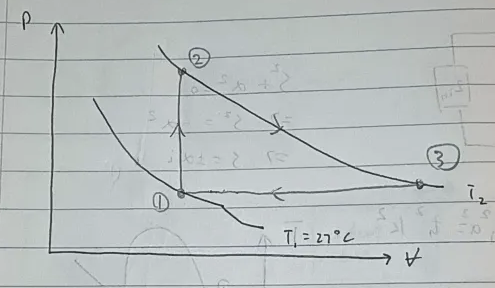
\includegraphics[width=0.7\textwidth]{9-13-2.png}
\end{center}
\textbf{Ratio of compression work to expansion work}\\
First, using the ideal gas law ($P\svol = RT$) to find the temperature at state 2. Since the process from state 1 to state 2 is a constant volume process, we have:
\[\frac{P_1}{T_1} = \frac{P_2}{T_2}=\frac{R}{\svol} \quad \text{(constant)}\]
\[\implies T_2 = \frac{P_2}{P_1}T_1 = \frac{[850\text{ kPa}]}{[100\text{ kPa}]} [27 + 273.15\text{ K}] = \underline{2551.275\text{ K}}\]
Since the process from state 2 to state 3 is an isothermal process:
\[T_3 = T_2 = \underline{2551.275\text{ K}}\]
There is isothermal expansion from state 2 to state 3, so the work done is given by:
\[W_{2\to3} = C\ln\left(\frac{\vol_3}{\vol_2}\right)\]
Where $C= RT_2$ is a constant. 
\[\implies w_{2\to3} = RT_2\ln\left(\frac{7\vol_2}{\vol_2}\right) = [0.287\text{ kJ/kg$\cdot$K}][2551.275\text{ K}]\ln(7) = 1427.82\text{ kJ/kg}\]
There is an isobaric compression from state 3 to state 1, so the work done is given by:
\[W_{3\to1} = P_1(\vol_1 - \vol_3) = mP_1(\svol_1 - \svol_3)\]
Where $\vol_3 = 7\vol_2 = 7\vol_1$. From the ideal gas law, we can find the specific volume at state 1:
\[P_1 \svol_1 = R T_1 \implies \svol_1 = \frac{R T_1}{P_1} = \frac{[0.287\text{ kJ/kg$\cdot$K}][27 + 273.15\text{ K}]}{[100\text{ kPa}]} = 0.8614\text{ m$^3$/kg}\]
Dividing by mass to get specific work:
\[\implies w_{3\to1} = [100\text{ kPa}][0.8614 - 7\cdot 0.8614\text{ m$^3$/kg}] = -518.84\text{ kJ/kg}\]
Finally, the ratio of compression work to expansion work is:
\[\left|\frac{w_{3\to1}}{w_{2\to3}}\right| = \left|\frac{-518.84}{1427.82}\right| = \boxed{0.363}\]
\textbf{Determine Thermal Efficiency}\\
The thermal efficiency of the cycle is given by:
\[\eta = \frac{W_{net}}{Q_{in}}\]
The net specific work on the system is:
\[w_{net} = w_{2\to3} + w_{3\to1} = 1427.82 - 518.84 = 908.98\text{ kJ/kg}\]
For the heat transfer, we start by looking process from states 1 to 2. Since this is a constant volume process, there is no work done. By the first law of thermodynamics:
\[\Delta U = Q - W \implies Q = \Delta U\]
\[\implies q_{1\to2} = u_2 - u_1 = c_{\svol} (T_2 - T_1)\]
\[q_{1\to2} = [0.718\text{ kJ/kg$\cdot$K}][2551.275 - 300.15\text{ K}] = 1616.307\text{ kJ/kg}\]
The process from state 2 to state 3 is an isothermal process, so the change in internal energy is zero ($du = c_{\svol} dT = 0$). Thus, by the first law of thermodynamics:
\[\Delta U = Q - W \implies Q = W\]
\[\implies q_{2\to3} = w_{2\to3} = 1427.82\text{ kJ/kg}\]
The process from state 3 to state 1 is an isobaric process, so by the first law of thermodynamics:
\[\Delta U = Q - W \implies Q = \Delta U + W\]
\[q_{3\to1} = u_1 - u_3 + P(\svol_1 - \svol_3) = h_1 - h_3\]
\[\implies q_{3\to1} = c_p (T_1 - T_3) = [1.005\text{ kJ/kg$\cdot$K}][300.15 - 2551.275\text{ K}] = -2262.53\text{ kJ/kg}\]
However, the heat input to the system is only during the process from state 1 to 2 and from state 2 to 3 (heat is lost during the process from state 3 to state 1), thus
\[q_{in} = q_{1\to2} + q_{2\to3} = 1616.307 + 1427.82 = 3044.127\text{ kJ/kg}\]
Finally, the thermal efficiency of the cycle is:
\[\eta = \frac{W_{net}}{Q_{in}} = \frac{908.98\text{ kJ/kg}}{3044.127\text{ kJ/kg}} = \boxed{0.298}\]

\end{document}